\begin{frame}
  \frametitle{Model optimization: MCMC and VI with Stan}
  Stan is a C++ package providing
  \begin{itemize}
  \item
    Full Bayesian statistical inference with MCMC sampling (HMC, NUTS as default)
  \item
    Approximate Bayesian Inference with variational inference (ADVI)
  \item
    Penalized maximum likelihood estimation with optimization (L-BFGS)
  \end{itemize}
  One advantage of Stan is the support of automatically differentiation. They
  provide Python, R, the command line and other interfaces. Stan supports
  multi-threading. It also provides partially support of GPU with limited functions.\\
\end{frame}

\begin{frame}{ADVI}
  In our case, we apply both MCMC and VI for model inference.
  \begin{itemize}
  \item
    Variational inference is much faster than MCMC, especially when facing large
    scale of scRNAseq data sets. The pure MCMC is too slow to get the result.
  \item
    ADVI, i.e., automatic differentiation variational inference
    \cite{kucukelbir2017automatic}, uses \myemph{mean-field (factorized) or full-rank
    Gaussian distributions} and the \myemph{one-to-one differentiable functions} to
    approximate the constrained continuous random variables.
  \item
    It uses stochastic gradient ascent with adaptive step-size sequence
    to optimize the \(ELBO\), which is equal to minimize the KL
    divergence between the approximated distributions and the posterior
    distributions of the latent variables.
  \end{itemize}
\end{frame}

\begin{frame}{ADVI: representation, target function, reparameterization, and optimization}
  \begin{figure}
    \centering
    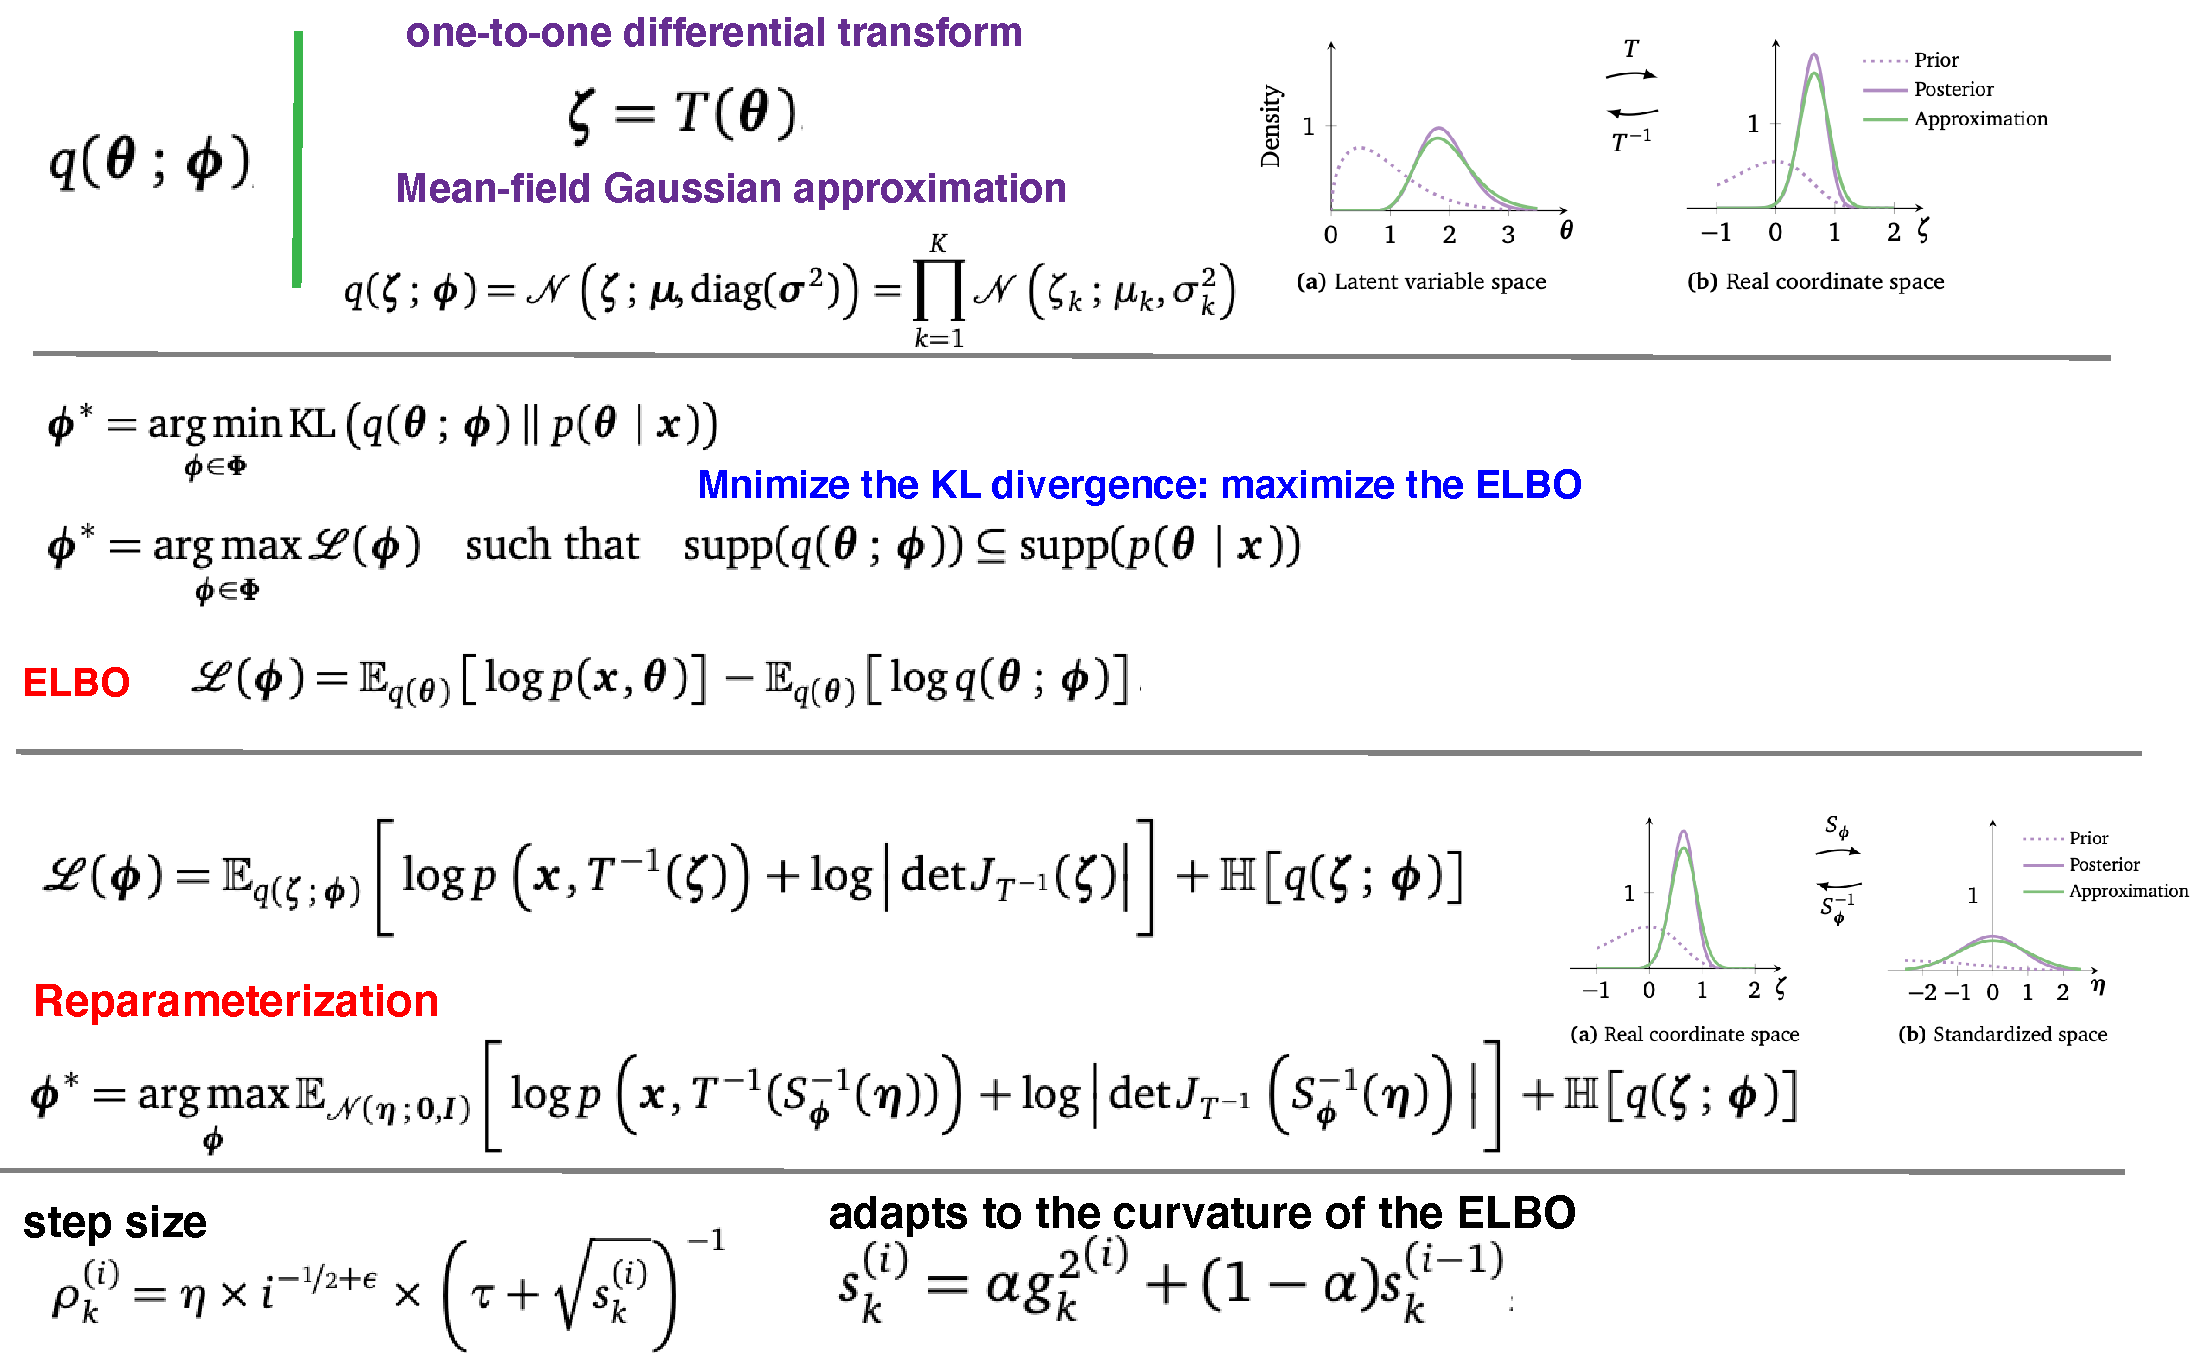
\includegraphics[width=0.9\textwidth]{advi}
  \end{figure}
\end{frame}
